\section{Reaching a flat endpoint with an infinite chain}
\label{sec:radial-tails}
\label{sec:radial-selection}

A finite collection of turning circles cannot produce the endpoint
behavior we need.  The construction instead repeats a small local
mechanism infinitely often.  On one part of each cell the solution has
almost constant value and its flux changes; on the next part its flux
is almost constant and its value changes.  The exact continuous equation
then has a discrete recurrence with a large diagonal.  Its decaying
solution loses approximately $e^{-2n^2}$ on crossing cell $n$.
Accumulating those losses gives $e^{-2n^3/3}$, fast enough to survive
every fixed number of derivatives in the shrinking radial intervals.

This section makes that picture precise.  We first build the actual
smooth profile, then derive the recurrence without discarding its error
terms.  Only after those estimates are established do we choose the
height ratios which prevent matching resonances.

\subsection{The budget of lengths, amplitudes and errors}

Let $d_n$ be the least nonsquare integer not smaller than $e^{n^2}$.
Then $d_n=e^{n^2}+O(1)$.  Use \eqref{eq:rad-eq-rm5} with this integer,
writing the resulting parameters $A_n$ and $B_n$; thus
$A_n\asymp e^{-n^2}$ and $B_n\asymp A_n^9$.
Initially let $\lambda_n=e^{-n^{5/2}}$.  Later we allow
\begin{equation}\label{eq:rad-eq-js2}
 \lambda_n=e^{-n^{5/2}}\prod_{k=N}^n\sigma_k,
 \qquad 1\le\sigma_k\le2.
\end{equation}
Their logarithms change by at most $O(n)$, which does not disturb the
scale comparisons below.

The choices can be understood before the details of the profile are
computed.  A finite-order derivative on a cell of size $e^{-n^2}$
costs $e^{C_sn^2}$.  Its amplitude must decay faster; the exponent
$n^{5/2}$ does this.  The solution itself must decay faster still in
order to pay for inverse coefficients.  Its cubic exponent will come
from the recurrence.  These requirements leave the interval
$2<5/2<3$, rather than singling out an optimal numerical exponent.

\begin{table}[htbp]
\centering
\begin{tabularx}{\linewidth}{@{}l l X@{}}
\toprule
Quantity & Size & Purpose\\
\midrule
Radial cell length & $A_n\asymp e^{-n^2}$ & Summable lengths at a finite endpoint.\\
Profile amplitude & $e^{-n^{5/2}+O(n)}$ & Flatness after every fixed derivative cost $e^{C_sn^2}$.\\
Positive joining length & $\asymp A_n^{12}$ & A large height change has negligible transfer error.\\
Allowed matching angle & $\delta_n=c_0e^{-n^2}$ & Summable bad sets over all frequency bands.\\
Solution attenuation & $e^{-S_n}$, $S_n=2n^3/3$ & Integrability and flat extension of the selected solution.\\
Coefficient allowance & $\mathcal E_n=e^{n^{5/2}\log(e+n)}$ & Absorbs fixed coefficient and coordinate losses while remaining smaller than $e^{\varepsilon S_n}$.\\
\bottomrule
\end{tabularx}
\caption{The scale choices are a budget for distinct jobs.  Their
compatibility is verified in the construction and recurrence below.}
\label{tab:endpoint-budget}
\end{table}

In particular, for fixed $a,b,\varepsilon>0$,
\begin{equation}\label{eq:rad-scale-separation}
 \mathcal E_n^a e^{bn^2}\le C_{a,b,\varepsilon}e^{\varepsilon S_n},
 \qquad n^2=o(q_n),\qquad q_n=o(S_n).
\end{equation}
These comparisons concern fixed derivative orders.  No assertion of
uniform bounds as the derivative order tends to infinity is being made.

\subsection{A cell of the actual radial profile}

On a Morse interval solve
\begin{equation}\label{eq:rad-eq-rm4}
 r_X=v>0,\qquad v_X=-\rho r,\qquad
 \rho=A(e^{-X}-e^{-2X})-B,\qquad w=\lambda v.
\end{equation}
The last identity in \eqref{eq:rad-eq-sc0} becomes
$L_j=-(\lambda/v)H_{j,M}$.  Let $X_R$ be the right zero of $\rho$.
Prescribe $r(X_R)=1$, $v(X_R)=\delta A^5$ with fixed small
$\delta>0$.  Retain the model from $X_c=-\log(3/2)$ to
$X_R+c_RA^{-4}$, for a fixed sufficiently small $c_R>0$.

Here are the estimates which ensure this is a genuine increasing
radius.  On $[X_c,X_R]$ the weighted integral of $|\rho|$ is $O(A)$,
so the reverse Volterra equation
\[
 r(X)=1-v(X_R)(X_R-X)
       -\int_X^{X_R}(Y-X)\rho(Y)r(Y)\,dY
\]
gives $r=1+O(A)$.  At the left cut it yields
\begin{equation}\label{eq:rad-eq-rm6a}
 v(X_c)=3A/8+O(A^2),\qquad
 r(X_c)=1-15A/16+O(A^2).
\end{equation}
The two leading integrals, after $t=e^{-X}$, are
$\int_0^{3/2}(1-t)\,dt=3/8$ and
$\int_0^{3/2}\log((3/2)/t)(1-t)\,dt=15/16$.
The constant $B$ contributes only $O(B\log^2(A/B))=o(A^2)$.
On the negative component, backward integration from $X_R$ keeps
$v$ positive; on the short left positive component its minimum is the
positive value at $X_c$.  On the long right positive component,
comparison with $r_{XX}=Br$ gives
\begin{equation}\label{eq:rad-eq-rm6}
 \begin{gathered}
 r=1+O(A),\qquad cA^5\le v\le CA,\qquad
 v\asymp A^5\text{ on the long right part},\\
 \Delta r\asymp A,\qquad
 \int_{X_c}^{X_R}v^2\,dX\asymp A^2,\qquad
 \int_{\text{each positive cap}}\sqrt{-\rho}\,dX\asymp\sqrt A.
 \end{gathered}
\end{equation}
For the last long-cap estimate use
$\sqrt B\,A^{-4}\asymp\sqrt A$; on the short cap
$-\rho\ge cA$ on a fixed subinterval.  Taking $c_R$ small ensures
that $r$ stays in a fixed positive range throughout this argument.

Multiply $r,v$ by a radius factor $\mathfrak r_n$.  To pass from a
cell to its next neighbor in the increasing-$r$ direction, insert a
positive interval of length
\begin{equation}\label{eq:rad-eq-rm7}
 \ell_{n,m}=c_Cr_o\min(A_n,A_m)^{12},\qquad m=n\pm1,
\end{equation}
where $r_o$ is its initial radius.  Choose the neighboring radius
factor so that its left endpoint is $r_o+\ell_{n,m}$.
The ratio of successive radius factors is $1+O(A_n+A_m)$.
The recursion converges on either end, with a prescribed limiting
radius on the left.  Thus the radii stay in a compact subset of
$(0,\infty)$ and all cells accumulate at finite endpoints.

At this joining interval the profile increases from $W_L$ to $W_R$,
with
\begin{equation}\label{eq:height-contrast-new}
 \log(W_R/W_L)=4n^2+O(n^{3/2}+n).
\end{equation}
To match the complete smooth germs, put $f=\log w$ and prescribe
\begin{equation}\label{eq:rad-eq-rm8}
 f'=\chi_Lf_L'+\chi_Rf_R'+C_1(1-\chi_L-\chi_R),
 \qquad
 C_1=\frac{\log(W_R/W_L)-\int\chi_Lf_L'-\int\chi_Rf_R'}
             {\int(1-\chi_L-\chi_R)}.
\end{equation}
The end cutoffs have disjoint supports and equal one near the respective
ends.  Their derivative integrals are
$O(\ell_{n,m}/\min(A_n,A_m))$, whereas the required logarithmic
height change is comparable to $n^2$.  Hence $C_1>0$ and, after the
fixed initial index is increased, $w'/w\ge2/r$ on the joining interval.
Integrating $f'$ with the left value matches the right value and all
endpoint derivatives.

This explains the apparently extravagant exponent $12$.
The height contrast costs $e^{4n^2+o(n^2)}$.  At the largest frequency
assigned to this cell, $j^2$ costs $e^{n^2}$ times a polynomial.
The interval length contributes $e^{-12n^2+o(n^2)}$.
Their product is $e^{-7n^2+o(n^2)}$, much smaller than the allowed
matching angle $e^{-n^2}$.  The same choice makes both the mass and
resistance of the join negligible in the estimates below.  No minimal
choice of this exponent is needed.

\paragraph{Flatness and coefficient bounds.}
The length of cell $n$ is comparable to $A_n$, and
$A_{n+1}/A_n=e^{-2n-1}(1+o(1))$.  If $d_\partial$ is distance to the
endpoint, then on that cell and its assigned joins
\begin{equation}\label{eq:geometry-endpoint-distance}
 cA_{n+1}\le d_\partial\le CA_n,
 \qquad \log(d_0/d_\partial)=n^2+O(n).
\end{equation}
All interval lengths and their reciprocals are bounded by $e^{Cn^2}$.
On a model, $\partial_r=v^{-1}\partial_X$ and $v\ge c\mathfrak r_nA_n^5$.
The differential equations for $r,v$ bound every fixed derivative of
$\log v$ by $e^{C_sn^2}$.  Formula~\eqref{eq:rad-eq-rm8} gives the
same bound on the joins.  Since each derivative of $e^{\pm\log w}$
contains only one undifferentiated exponential, we obtain
\begin{equation}\label{eq:geometry-profile-jets}
 \begin{gathered}
 e^{-n^{5/2}-Cn^2}\le w\le e^{-n^{5/2}+Cn^2},\\
 |\partial_r^sw|\le C_se^{-n^{5/2}+C_sn^2},\qquad
 |\partial_r^s(w^{-1})|\le C_se^{n^{5/2}+C_sn^2}.
 \end{gathered}
\end{equation}
Comparison with \eqref{eq:geometry-endpoint-distance} proves that
extension by zero is smooth and flat.  It also proves the fixed-order
coefficient bounds in Definition~\ref{def:radial-weights}, uniformly in
all height choices \eqref{eq:rad-eq-js2}.

\subsection{Why a mass--resistance chain appears}

Use $y=\log r$.  For the mode-two comparison density
$\mathsf p=wr^7$, divide a cell into a mass interval $I_n$ (the short
positive cap and the negative component) and a resistance interval
$J_n$ (the long positive cap and its following short join).  Define
\begin{equation}\label{eq:mass-resistance-def-new}
 \mu_n=\int_{I_n}\mathsf p\,dy,\quad
 R_n^I=\int_{I_n}\mathsf p^{-1}\,dy,\quad
 \nu_n=\int_{J_n}\mathsf p\,dy,\quad
 R_n=\int_{J_n}\mathsf p^{-1}\,dy.
\end{equation}
For an equation $-(\mathsf p V_y)_y=\Lambda\mathsf p V$, the change
of flux across an almost constant-value region is its value times
$-\Lambda$ times the mass.  The change of value across an almost
constant-flux region is the flux times the resistance.  This gives the
picture in Figure~\ref{fig:mass-resistance-chain}; the estimates following
it turn the picture into an exact reduction.

\begin{figure}[htbp]
\centering
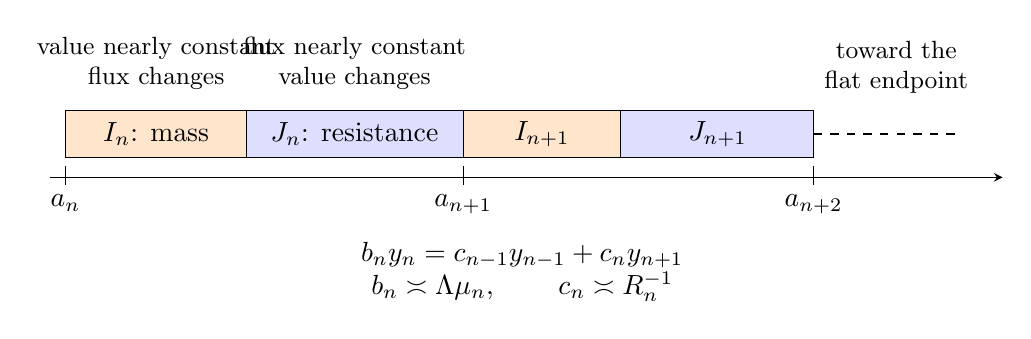
\begin{tikzpicture}[x=1cm,y=1cm,>=stealth]
\draw[->] (0,0)--(12.1,0);
\node[align=center,font=\small] at (10.75,1.4)
 {toward the\\flat endpoint};
\draw[fill=orange!20] (.2,.25) rectangle (2.5,.85);
\draw[fill=blue!13] (2.5,.25) rectangle (5.25,.85);
\draw[fill=orange!20] (5.25,.25) rectangle (7.25,.85);
\draw[fill=blue!13] (7.25,.25) rectangle (9.7,.85);
\draw[dashed] (9.7,.55)--(11.5,.55);
\node at (1.35,.55) {$I_n$: mass};
\node at (3.87,.55) {$J_n$: resistance};
\node at (6.25,.55) {$I_{n+1}$};
\node at (8.48,.55) {$J_{n+1}$};
\foreach \x/\lab in {.2/a_n,5.25/a_{n+1},9.7/a_{n+2}}
 {\draw (\x,-.1)--(\x,.15);\node[below] at (\x,-.1) {$\lab$};}
\node[align=center,font=\small] at (1.35,1.45) {value nearly constant\\flux changes};
\node[align=center,font=\small] at (3.87,1.45) {flux nearly constant\\value changes};
\node[align=center] at (6,-1.2)
 {$b_n y_n=c_{n-1}y_{n-1}+c_ny_{n+1}$\\
 $b_n\asymp\Lambda\mu_n$, \qquad $c_n\asymp R_n^{-1}$};
\end{tikzpicture}
\caption{The continuous intervals and their exact node equation.
The drawing is schematic; $a_n=(-1)^ny_n$ for the decaying solution.
Large products $\Lambda\mu_nR_n$ make successive node values small.}
\label{fig:mass-resistance-chain}
\end{figure}

Since $dr=v\,dX$, the two measures in
\eqref{eq:mass-resistance-def-new} are $wr^6dr$ and $dr/(wr^8)$.
Using \eqref{eq:rad-eq-rm6} gives
\begin{equation}\label{eq:rad-eq-rm10}
 \mu_n\asymp\lambda_nA_n^2,\qquad
 R_n^I\le C\lambda_n^{-1}\log(A_n/B_n),\qquad
 \nu_n\le C\lambda_nA_n^6,\qquad
 R_n\asymp\lambda_n^{-1}A_n^{-4}.
\end{equation}
A radius dilation multiplies the mass by its eighth power and the
resistance by its inverse eighth power; the products below are unchanged.
The joining interval contributes at most $W_R\ell$ to mass and
$\ell/W_L$ to resistance.  Their relative errors are respectively
$e^{-7n^2+O(n^{3/2}+n)}$ and $e^{-11n^2+O(n)}$, so
\begin{equation}\label{eq:rad-eq-rm11}
 \mu_nR_n\asymp A_n^{-2},\qquad
 \mu_nR_n^I\le CA_n^2\log(A_n/B_n),\qquad
 \nu_nR_n\le CA_n^2,
\end{equation}
while
\begin{equation}\label{eq:rad-eq-rm12}
 \log(\mu_{n+1}R_n)=2n^2+O(n^{3/2}+n).
\end{equation}

The same structure handles a general frequency.  The exact gauge
$u=r^{j^2}V$ gives
\begin{equation}\label{eq:rad-eq-rm13}
 (\mathsf p_jV_y)_y+\Lambda\mathsf p_jV=0,
 \qquad \mathsf p_j=wr^{2j^2-1},\qquad \Lambda=j^2(j^2-1).
\end{equation}
After removing its constant endpoint factor,
$\mathsf p_j/\mathsf p=(r/r_\partial)^{2(j^2-4)}$.
On the tail beyond $N$ its logarithm is bounded by $Cj^2A_N$.
Thus the mass and resistance comparisons remain uniform whenever
$j^2A_N$ is bounded.  The stronger condition used below is
\begin{equation}\label{eq:deep-frequency-condition-new}
 j^2A_N\sqrt{\log(A_N/B_N)}\le c.
\end{equation}

\subsection{The exact continuous-to-discrete reduction}

Orient $x=\log r$ on the right and $x=-\log r$ on the left, so $x$
always increases toward the flat endpoint.  On the left the outward
order is $J_N,I_N,J_{N+1},I_{N+1},\ldots$; therefore, within this
reduction only, the resistance following $I_n$ is the original
$J_{n+1}$.  This one-index change affects only the lower-order terms
in \eqref{eq:rad-eq-rm12}.  The initial $J_N$ is treated as a separate
resistance edge.

The following conditions isolate precisely what is needed from the
profile.  For a positive density $\mathsf p$, assume
\begin{equation}\label{eq:rad-eq-dg1}
 \begin{gathered}
 \Lambda\mu_nR_n^I+\Lambda\nu_nR_n\le\eta\ll1,\qquad
 \Lambda\mu_nR_n,\ \Lambda\mu_{n+1}R_n\ge K\gg1,\\
 \nu_n\le\eta\min(\mu_n,\mu_{n+1}).
 \end{gathered}
\end{equation}
An initial resistance edge has the same large-product conditions and
$\Lambda\nu_0R_0\le\eta$, $\nu_0\le\eta\mu_N$.
Call this a \emph{deep tail}.  Equations
\eqref{eq:rad-eq-rm10}--\eqref{eq:deep-frequency-condition-new} imply
these conditions for $\mathsf p_j$ after the initial index is large
enough.

\begin{lemma}[Deep inverse and unique decaying line]
\label{lem:radial-deep-inverse}
\label{lem:radial-flat-line}
On a deep tail let
$A_{\mathsf p}=-\mathsf p^{-1}(\mathsf p\partial_x)'$ act in
$\mathcal H=L^2(\mathsf p\,dx)$, with Dirichlet condition at the finite
entrance and the Friedrichs condition at the outer endpoint.  Then
\[
 \|(A_{\mathsf p}-\Lambda)^{-1}\|\le C/\Lambda.
\]
The homogeneous equation has exactly one square-integrable line at
the outer endpoint.  At successive mass entrances its nonzero values
are $a_n=(-1)^ny_n$, with $y_n>0$ and
\begin{equation}\label{eq:rad-eq-dg4}
 \frac{y_{n+1}}{y_n}
 =\frac{1+O(\eta)+O(K^{-1})}{\Lambda\mu_{n+1}R_n},
 \qquad
 \frac{\sqrt{\mu_{n+1}}y_{n+1}}{\sqrt{\mu_n}y_n}\le C/K<1/2.
\end{equation}
For the constructed Morse tails this line, transferred back to $u$,
is smooth and flat in the original radius.
\end{lemma}

\begin{proof}
We give the reduction on the continuous equation, so that the endpoint
condition and the operator norm follow from the same argument.
Introduce resistance coordinate $ds=dx/\mathsf p$ on an edge
$E_n=I_n\cup J_n$.  Its length is $L_n=R_n^I+R_n$ and its density is
$\omega=\mathsf p^2$, so $\mathsf p\,dx=\omega\,ds$ and
\[
 (A_{\mathsf p}-\Lambda)u=f
 \quad\Longleftrightarrow\quad -u_{ss}-\Lambda\omega u=\omega f.
\]
The zero-potential Dirichlet kernel is
$G_0(s,t)=\min(s,t)[L_n-\max(s,t)]/L_n$.
The small quantity in this equation is
\[
 \delta_n^{\rm edge}=\Lambda\int\omega(s)G_0(s,s)\,ds\le3\eta,
 \qquad R_n^I/L_n\le\eta/K.
\]
The kernel inequality
$G_0(s,z)G_0(z,t)\le G_0(s,t)G_0(z,z)$ bounds its resolvent series
term by term.  Hence the actual kernel and the two boundary-height
functions satisfy
\begin{equation}\label{eq:rad-eq-dg2}
 G_0\le G_\Lambda\le(1-\delta_n^{\rm edge})^{-1}G_0,
 \qquad l_i\le v_i\le(1-\delta_n^{\rm edge})^{-1}l_i,
 \quad l_0=1-s/L_n, l_1=s/L_n.
\end{equation}
The analogous inequality for the Poisson functions follows by replacing
one kernel factor by $l_i$.  For a zero-boundary $u$,
$\Lambda\int\omega|u|^2\le\delta_n^{\rm edge}\int|u_s|^2$.
Thus the direct sum $G_D$ of the Dirichlet edge inverses has norm
at most $C\eta/\Lambda$.

The outward derivative matrix of this exact edge problem is
\[
 \begin{pmatrix}d_{n,0}&-c_n\\-c_n&d_{n,1}\end{pmatrix},\qquad
 c_n=L_n^{-1}+\Lambda\int\omega l_0v_1,\qquad
 d_{n,i}=L_n^{-1}-\Lambda\int\omega l_iv_i.
\]
Since $l_0l_1=G_0(s,s)/L_n$, we have
\begin{equation}\label{eq:rad-eq-dg3}
 c_n=R_n^{-1}(1+O(\eta)),\qquad
 b_n:=-d_{n-1,1}-d_{n,0}
       =\Lambda\mu_n(1+O(\eta)+O(K^{-1})).
\end{equation}
For the second estimate, the mass on $I_n$ sees
$l_0=1+O(R_n^I/L_n)$.  The preceding edge contributes at most
$\nu_{n-1}+\mu_{n-1}(R_{n-1}^I/L_{n-1})^2$; the second term is
at most $\eta^2K^{-2}\mu_n$ by \eqref{eq:rad-eq-dg1}.
The two $L^{-1}$ terms are at most $2\Lambda\mu_n/K$.
These calculations also cover the initial resistance edge.

For node values $a=(a_n)$ put
$(Ta)|_{E_n}=a_nv_0+a_{n+1}v_1$ and let
$\mathfrak h=\ell^2(\mu_n)$.  Equation~\eqref{eq:rad-eq-dg2} gives
\begin{equation}\label{eq:rad-eq-dj1}
 c\|a\|_{\mathfrak h}^2\le\|Ta\|_{\mathcal H}^2
                         \le C\|a\|_{\mathfrak h}^2.
\end{equation}
For example, on $I_n$ the squared neighbor term costs at most
$C\mu_n(R_n^I/L_n)^2|a_{n+1}|^2$; after an index shift its sum is
$O(\eta^2/K^2)\|a\|_{\mathfrak h}^2$.  The mass of $J_n$ is handled
by its last inequality in \eqref{eq:rad-eq-dg1}.

The shifted quadratic form on these interpolants is
\[
 (\mathcal Da,a)_{\mathfrak h}
   =-\sum b_n|a_n|^2-2\operatorname{Re}\sum c_na_n\overline{a_{n+1}}.
\]
In coordinates $\sqrt{\mu_n}a_n$, the diagonal has size $\Lambda$,
while each of the two neighboring entries is bounded by
$C/(R_n\sqrt{\mu_n\mu_{n+1}})\le C\Lambda/K$.
Diagonal dominance therefore gives
$\|\mathcal D^{-1}\|\le C/\Lambda$, independently of the number
of edges.

These algebraic formulas give an operator inverse because they respect
the form domain.  The interpolation energy is bounded by
$C\Lambda\|a\|_{\mathfrak h}^2$ using its shifted form and
\eqref{eq:rad-eq-dj1}.  Conversely, averaging $u(x_n)-u(x)$ on
$I_n$ gives
\[
 \mu_n|u(x_n)|^2\le2\|u\|_{I_n}^2+
             2\mu_nR_n^I\int_{I_n}|u_s|^2.
\]
Thus every form-domain function has square-summable node data and
splits as $Ta+v$, where $v$ vanishes at every node.  The two parts
are orthogonal for the shifted form, by the homogeneous edge equation.
Consequently the exact inverse is
\begin{equation}\label{eq:rad-eq-dj2}
 (A_{\mathsf p}-\Lambda)^{-1}=G_D+T\mathcal D^{-1}T^*,
 \qquad (T^*f)_n=\mu_n^{-1}\int\mathsf p\,(T\mathbf e_n)f\,dx.
\end{equation}
Finite Dirichlet truncations have this same formula and converge
strongly: the uniformly convergent diagonal resolvent series for
$\mathcal D^{-1}$ converges on finite compressions, and the direct edge
terms do as well.  Their limit is the Friedrichs realization just
identified by the form decomposition.  This proves the inverse bound.

For the homogeneous line, substituting $a_n=(-1)^ny_n$ gives
$b_ny_n=c_{n-1}y_{n-1}+c_ny_{n+1}$.
Set $\epsilon_n=c_n^2/(b_nb_{n+1})\le C/K^2$ and
$t_n=b_{n+1}y_{n+1}/(c_ny_n)$.  Backward elimination is
\[
 t_n=(1-\epsilon_{n+1}t_{n+1})^{-1}.
\]
For large $K$ these maps preserve $[1,2]$ and contract by at most
$1/2$.  Finite outer walls therefore give a unique bounded limiting
sequence.  Equation~\eqref{eq:rad-eq-dg3} yields
\eqref{eq:rad-eq-dg4}, and \eqref{eq:rad-eq-dj1} makes its
interpolation square integrable.
An independent node solution has the Wronskian form
\[
 z_n=y_n\left(C+\mathcal W\sum_{k=N}^{n-1}
                \frac1{c_ky_ky_{k+1}}\right),\qquad\mathcal W\ne0.
\]
Successive summands grow by at least $cK^2$, so eventually
$|z_{n+1}/z_n|\asymp\Lambda\mu_nR_n$ and
$\sqrt{\mu_{n+1}}|z_{n+1}|\ge cK\sqrt{\mu_n}|z_n|$.
On the mass interval its neighbor term is at most $C\eta$ times its
own-node term.  Its continuous $L^2$ mass therefore diverges.
This proves uniqueness of the square-integrable line and the
limit-point property.

Finally, summing \eqref{eq:rad-eq-rm12} in
\eqref{eq:rad-eq-dg4} gives, for $k\ge m$,
\begin{equation}\label{eq:rad-eq-rm17}
 \left|\frac{a_k}{a_m}\right|
 \le\mathcal E_k^C\mathcal E_m^C e^{-(S_k-S_m)},\qquad
 2\sum_{n=m}^{k-1}n^2
 =\frac23(k^3-m^3)-(k^2-m^2)+\frac13(k-m).
\end{equation}
The accumulated $O(n^{3/2}+n)$ error is absorbed by $q_k+q_m$.
Every fixed radial derivative costs at most $e^{C_sn^2}$, by the
profile equation and the interval lengths.  The normalized gauge
$(r/r_\partial)^{j^2}$ is bounded with bounded inverse in the deep
range.  Thus the constructed homogeneous solution and all its fixed
radial derivatives are bounded by $\mathcal E_n^{C_s}e^{-S_n}$
after a fixed entrance normalization.  They extend flatly at the
endpoint.  The same contraction also shows continuity of the endpoint
line in the product topology of all the height ratios.
\end{proof}

\paragraph{The localized Green estimate.}
We will use a little more than the operator norm.  Let $B$ be the
positive node matrix with diagonal $b_n$ and neighboring entries
$-c_n$, and let $W=\operatorname{diag}(\mu_n)$.
Define
$\Gamma_{nm}=(\mu_n\mu_m)^{-1/2}
 (W^{-1/2}BW^{-1/2})^{-1}_{nm}$.
Its diagonal lies between $b_m^{-1}$ and $Cb_m^{-1}$ by the
positive diagonal series.  Uniqueness of the decaying recurrence gives
\begin{equation}\label{eq:rad-eq-dj4}
 \Gamma_{nm}=\Gamma_{mm}\frac{y_n}{y_m}
 \le\frac{C}{\Lambda\mu_m}
      \prod_{k=m}^{n-1}\frac{1+C(\eta+K^{-1})}{\Lambda\mu_{k+1}R_k}
 \quad(n\ge m).
\end{equation}
Symmetry handles the reverse direction.  The interpolation kernel in
\eqref{eq:rad-eq-dj2} has the additional sign $-(-1)^{n+m}$, which
is irrelevant to absolute estimates.  The continuous kernel adds the
same-edge Dirichlet term and at most two interpolation functions at
each endpoint.  Hence its localized absolute bound is
\begin{equation}\label{eq:rad-eq-dj5}
 C\mathcal E_n^C\mathcal E_m^C e^{-|S_n-S_m|}.
\end{equation}
For the original source convention, put
$g=(r/r_\partial)^{j^2}$ and $\mathsf p^\circ=g^2w/r$.
A direct calculation gives
\[
 L_j(gV)=-\frac{gw}{r^2}(A_{\mathsf p^\circ}-\Lambda)V,
 \qquad \mathsf p^\circ dx=\frac{g^2w}{r^2}\,dr,
 \qquad G_{L_j}(r,r')=-g(r)g(r')G_A(x,x').
\]
The bounded gauge factors preserve \eqref{eq:rad-eq-dj5} in the
$dr$ pairing.  Also, for $B_j=-\varpi^{-1}L_j$,
\begin{equation}\label{eq:rad-eq-rm20}
 B_j=\frac1{12}(A_{\mathsf p_j}-j^2(j^2-1)),
 \qquad \|B_{j,D}^{-1}\|\le Cj^{-4}
\end{equation}
on a deep tail.  At its entrance the derivative matrix gives
$\mathsf p u_x/(\Lambda\mu_nu)=1+O(\eta)+O(K^{-1})$.
If an initial resistance edge comes first, the impedance is instead
$-(1+O(\eta)+O(K^{-1}))/R_0$.  In either case the endpoint
Green pairing vanishes: at the nodes it is bounded by
$C\Lambda\mu_n|a_n|^2\to0$, and finite mass and energy identify this
with the endpoint limit.

\subsection{One transition cell at every frequency}

The useful decomposition depends on frequency, although the geometry
does not.  Put
\begin{equation}\label{eq:rad-eq-rm21}
 \mathcal H_n=C_*q_nA_n^{-1/2},\qquad
 \mathcal I_n=\{j:\mathcal H_{n-1}\le j<\mathcal H_n\}.
\end{equation}
At the initial index $N$, include every remaining even frequency
$2\le j<\mathcal H_N$ in the first band.  For $j\in\mathcal I_n$,
all earlier cells have large positive-cap action
$j\sqrt{A_m}\ge C_*q_m$.  Cell $n$ is the transition cell; the
next one is already deep, since
\begin{equation}\label{eq:rad-eq-rm22}
 j^2A_{n+1}\sqrt{\log(A_{n+1}/B_{n+1})}
 \le Cq_n^2(A_{n+1}/A_n)(n+1)\longrightarrow0.
\end{equation}
Thus there is no unexamined frequency range between the local model
inverse and the deep inverse.  This one-transition-cell decomposition
will be crucial when the inverse is assembled.

At each finite tail entrance attach an auxiliary positive cone $w=cr$.
For the right tail it continues to $r=0$, and for the left tail to
$r=\infty$.  A short positive interpolation with $rw'/w\ge1$ is
constructed by applying \eqref{eq:rad-eq-rm8} to $\log(w/r)$.
The cone merely specifies an incoming line.  The final surface retains
only a finite piece of it.  In $y=\log r$,
\[
 B_j=\tfrac1{12}(-\partial_y^2+j^2),\qquad
 \varpi\,dr=12c\,dy;
\]
the incoming lines are $r^j$ and $r^{-j}$ respectively, and the
Dirichlet inverse has norm at most $12/j^2$.

\subsection{Choosing the heights so that the lines do not meet}

For $j\in\mathcal I_n$, select the positive join immediately before
cell $n$ in the outward order.  Its inner height $W_{\rm in}$ does
not depend on $\sigma_n$, while its outer height is
$\sigma_nW_{\rm out}^0$.  Write
\begin{equation}\label{eq:rad-eq-js4}
 \Xi_n=W_{\rm out}^0/W_{\rm in},\qquad
 \Upsilon_n=\max(\Xi_n,\Xi_n^{-1}),\qquad
 \log\Upsilon_n=4n^2+O(n^{3/2}+n).
\end{equation}
The radius recursion and all cut locations are independent of the height
choices.  At the first join choose the auxiliary cone amplitude
independently of $\sigma_N$, with the same contrast as in
\eqref{eq:rad-eq-js4}.
All later pieces are multiplied by the same $\sigma_n$, so their
homogeneous equations, and hence their natural endpoint line, are
unchanged.  The incoming line is determined before this join and is
also independent of $\sigma_n$.  What changes is the flux scale by
which the two lines are compared.

We first control the incoming slope.  Set
\begin{equation}\label{eq:rad-eq-js5}
 \zeta_j=ru_r/j^2-u.
\end{equation}
The solution coming from a Dirichlet cut in the preceding positive cap
can be normalized to $u=1$ at the join, and then
\begin{equation}\label{eq:rad-eq-js6}
 a:=\zeta_j/u\in[-3/2,-1/2].
\end{equation}
Indeed on that cap $u_{XX}=j^2|\rho|u$.
Comparison of $u_X/u$ with the constant-potential Riccati solution
gives
$|u_X/u|\le Cj\sqrt b\coth(cj\sqrt A)$, where the cap scales are
$(b,h,v)\asymp(A,1,A)$ or $(A^9,A^{-4},A^5)$.
In both cases $h\sqrt b\asymp\sqrt A$ and
$v\asymp\sqrt{Ab}$, so
$|ru_r/(j^2u)|\le C/(j\sqrt{A_{n-1}})<1/2$ after choosing $C_*$
large.  Reversing the left orientation changes only the sign.
In the first band the cone gives $ru_r/(j^2u)=\pm1/j$, proving the
same assertion even at $j=2$.

The derivative $w'/w$ can be very large on the short join.  It disappears
from the transfer equation if we use the right state.  The identity
$(w\zeta_j)'=-(j^2-1)wu_r/j^2$ gives, for
$Y=(u,w\zeta_j/W_{\rm in})$,
\begin{equation}\label{eq:rad-eq-js7}
 Y_r=\frac1r
 \begin{pmatrix}
 j^2&j^2W_{\rm in}/w\\
 -(j^2-1)w/W_{\rm in}&-(j^2-1)
 \end{pmatrix}Y.
\end{equation}
The transfer therefore differs from the identity by at most
$e^{\eta_{n,j}}-1$, where
\begin{equation}\label{eq:rad-eq-js14}
 \eta_{n,j}=Cj^2(\ell_n/r_{\min})\Upsilon_n
 \le CC_*^2q_n^2e^{-7n^2+O(n^{3/2}+n)}=o(e^{-n^2}).
\end{equation}
This follows directly from the Volterra series for the displayed
first-order system.  It uses only the size of $w$ and $w^{-1}$,
which is why the sharp interpolation causes no difficulty here.

\begin{figure}[htbp]
\centering
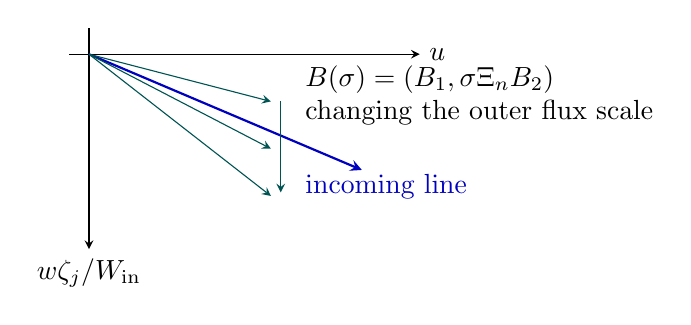
\begin{tikzpicture}[x=2.1cm,y=1.5cm,>=stealth]
\draw[->] (-.12,0)--(2,0) node[right] {$u$};
\draw[->] (0,.22)--(0,-1.65) node[below] {$w\zeta_j/W_{\rm in}$};
\draw[thick,blue!75!black,->] (0,0)--(1.65,-.98);
\node[anchor=west,blue!75!black] at (1.25,-1.12) {incoming line};
\draw[teal!65!black,->] (0,0)--(1.1,-.4);
\draw[teal!65!black,->] (0,0)--(1.1,-.8);
\draw[teal!65!black,->] (0,0)--(1.1,-1.2);
\draw[->,teal!65!black] (1.16,-.4)--(1.16,-1.17);
\node[anchor=west,align=left] at (1.25,-.35)
 {$B(\sigma)=(B_1,\sigma\Xi_nB_2)$\\changing the outer flux scale};
\end{tikzpicture}
\caption{Height selection in the two-dimensional boundary-state plane.
The incoming slope stays in a fixed negative interval.  A small angle
can therefore occur only for a short interval of the height parameter,
even when the height contrast $\Xi_n$ is very large or very small.}
\label{fig:height-selection}
\end{figure}

Normalize the natural endpoint line in its local $(u,\zeta_j)$ frame
to $(B_1,B_2)$.  In the common frame it is
$B(\sigma)=(B_1,\sigma\Xi_nB_2)$; this is the geometric content of
Figure~\ref{fig:height-selection}.  If $B_1=0$, its angle with
$(1,a)$ is bounded below.  Otherwise write
$b_\sigma=\sigma\Xi_nB_2/B_1$.  The ideal angle sine is
\[
 \frac{|a-b_\sigma|}{\sqrt{1+a^2}\sqrt{1+b_\sigma^2}}.
\]
A small value forces $b_\sigma$ into a fixed negative compact interval,
where $|b_\sigma'|=|b_\sigma|/\sigma$ is bounded below.  Thus the set
where this angle is less than $2\delta_n$, with
$\delta_n=c_0e^{-n^2}$, lies in an interval of length at most
$C\delta_n$.  The true incoming state is $(1,a)+O(\eta_{n,j})$;
normalization is Lipschitz near these vectors.  Equation
\eqref{eq:rad-eq-js14} therefore gives the same excluded-interval bound
for a true matching angle below $\delta_n$.
All constants are independent of the other height ratios.

\begin{lemma}[Simultaneous height selection]\label{lem:radial-product-selection}
At each endpoint one can choose all $\sigma_n\in[1,2]$ so that for
every even $j\in\mathcal I_n$ the incoming and natural endpoint
lines have angle sine at least $\delta_n=c_0e^{-n^2}$ in the common
state of \eqref{eq:rad-eq-js7}.
\end{lemma}
\begin{proof}
The union of the excluded sets has measure less than one, because
\begin{equation}\label{eq:rad-eq-js13}
 \sum_{n\ge N}C\#\mathcal I_n\delta_n
 \le CC_*c_0\sum_{n\ge N}q_ne^{-n^2/2}<\tfrac12
\end{equation}
for sufficiently large $N$.
More explicitly, for a finite set of bands fix all later ratios to one
and use Lebesgue measure on the finite cube of remaining ratios.
Fubini's theorem applies the uniform one-coordinate exclusion estimate
to each condition, and the union bound gives a good choice.
Extend those finite choices by ones and take a coordinatewise convergent
subsequence.  At any fixed frequency the finite-prefix transfer is
continuous, and the deep continued fraction proved above contracts
uniformly over all height choices.  Hence the natural line is continuous
in the product topology.  Each good-angle condition is closed and
survives the limit.  The two endpoints can be chosen independently.
\end{proof}

We have now constructed smooth flat tails with a quantitative endpoint
line at every frequency.  We have not yet claimed that gluing them to
the central oscillator preserves all the spectral gaps.  That global
question is addressed next.  Its answer uses both parts of the present
construction: the selected angle at the transition cell, and the strong
attenuation through the preceding positive cap.
